\documentclass[boxes,pages]{homework}

\name{Nate Stemen}
\studentid{20906566}
\email{nate.stemen@uwaterloo.ca}
\term{Fall 2020}
\course{Numerical Analysis}
\courseid{AMATH 740}
\hwnum{}
\duedate{Mon, Dec 14, 2020 4:30 PM}

\hwname{Final Exam}

\newcommand{\eqorder}[1]{\overset{h^#1}{=}}
\newcommand{\tpose}[1]{#1^\intercal}
\newcommand{\e}{\mathrm{e}}

\begin{document}

\begin{problem}
\begin{parts}
	\part{Consider the absolute values of the eigenvalues of $A$. Approximately, for large $n$, what is the largest eigenvalue (in absolute value) of $A$? What is, approximately, the smallest eigenvalue (in absolute value) of $A$, for large $n$?}\label{part:1a}
	\part{Approximately, for large $n$, what is the 2-norm condition number of $A$? What is its order as a function of $h$, and as a function of $n$? (Remember that $A$ is symmetric, so make sure to use the appropriate formula for the 2-norm condition number.)}\label{part:1b}
\end{parts}
\end{problem}

\begin{solution}
	\ref{part:1a}
	We start with the fact that the $\sin^2(x)$ function attains it's maximum (for positive $x$) at $x\in\{\frac{\pi}{2}, \frac{3\pi}{2},\ldots\}$. Now unfortunately because $k,l\in\{1,\ldots, N\}$, we can never actually attain any of these values because $\frac{k\pi}{2(N+1)} < \frac{\pi}{2}$. That said for large $N$ we have $N\approx N + 1$, so if we take $k$ to be $N$ then $\frac{k\pi}{2(N+1)} \approx \frac{\pi}{2}$. Hence, for the largest eigenvalue we take $k = N = l$.
	\begin{equation*}
		\abs{\lambda_\text{max}} = \abs{\lambda_{N, N}} = 4\qty[\sin^2\qty(\frac{N\pi}{2(N+1)}) + \sin^2\qty(\frac{N\pi}{2(N+1)})] = 8\sin^2\qty(\frac{N\pi}{2(N+1)})
	\end{equation*}
	For the smallest eigenvalue, we know $\sin^2(x)$ attains it's minimum (again for positive $x$) at $x\in\{0, \pi,\ldots\}$, but as we saw above, the argument to $\sin^2(x)$ is bounded above by $\frac{\pi}{2}$, so we opt to get as close to the $x = 0$ minimum. To do this we take $k = 1 = l$.
	\begin{equation*}
		\abs{\lambda_\text{min}} = \abs{\lambda_{1, 1}} = 4\qty[\sin^2\qty(\frac{\pi}{2(N+1)}) + \sin^2\qty(\frac{\pi}{2(N+1)})] = 8\sin^2\qty(\frac{\pi}{2(N+1)})
	\end{equation*}
	Now for more approximations. In $\abs{\lambda_\text{max}}$, when $N$ is \emph{very} large, we should always be very close to the maximum of $\sin^2(x)$ which is 1, so we can say $\abs{\lambda_\text{max}}\approx 8$. For $\abs{\lambda_\text{min}}$ we know we are working with a $\sin(x)$ function near 0, and hence we use the classic $\sin(x)\approx x + \order{x^3}$ Taylor approximation, but squaring both sides to say $\sin^2(x)\approx x^2 + \order{x^4}$. Thus we have $\abs{\lambda_\text{min}}\approx \frac{2\pi^2}{(N + 1)^2}$.

	\ref{part:1b}
	Now to calculate the 2-norm condition number we use the fact that it can be written as the ratio of the largest eigenvalue to the smallest.
	\begin{equation*}
		\kappa_2(A) = \frac{\abs{\lambda_\text{max}}}{\abs{\lambda_\text{min}}} = \frac{8}{\frac{2\pi^2}{(N + 1)^2}} = \frac{4(N+1)^2}{\pi^2} = \underbrace{\frac{4}{\pi^2}\qty(n + 2\sqrt{n}+ 1)}_{\order{n}} = \underbrace{\frac{4}{\pi^2h^2}}_{\order{h^{-2}}}
	\end{equation*}
\end{solution}

\begin{problem}
\begin{parts}
	\part{Write the update formula in vector form (using the decomposition $A = A_D - A_L - A_U$).}\label{part:2a}
	\part{Rewrite the vector form in the standard form of the update formula for a one-step, stationary iterative method, \[\vb{x}_{k+1} = \vb{x}_k + P\vb{r}_k,\] to show that the preconditioning matrix $P$ for SOR is given by \[P = \omega(A_D - \omega A_L)^{-1}.\]}\label{part:2b}
\end{parts}
\end{problem}

\begin{solution}
	\ref{part:2a},\ref{part:2b}
	Here we'll take a crack at both parts in one go. If you want, the first line of the sequence can be taken to be the solution to part (a), and the rest part (b).
	\begin{align*}
		\vb{x}_{k+1}                             & = (1 - \omega)\vb{x}_k + \omega A_D^{-1}\qty(\vb{b} + A_L\vb{x}_{k+1} + A_U\vb{x}_k)                           \\
		A_D\vb{x}_{k+1}                          & = (1 - \omega)A_D\vb{x}_{k} + \omega\qty(\vb{b} + A_L\vb{x}_{k+1} + A_U\vb{x}_k)                               \\
		A_D\vb{x}_{k+1} - \omega A_L\vb{x}_{k+1} & = (1 - \omega)A_D\vb{x}_{k} + \omega\vb{b} + \omega A_U\vb{x}_k                                                \\
		\qty(A_D - \omega A_L)\vb{x}_{k+1}       & =\qty[(1 - \omega)A_D + \omega(A_D - A_L - A)]\vb{x}_k + \omega\vb{b}                                          \\
		                                         & = A_D\vb{x}_k - \omega A_D\vb{x}_k + \omega A_D\vb{x}_k - \omega A_L\vb{x}_k - \omega A\vb{x}_k + \omega\vb{b} \\
		                                         & = \qty(A_D - \omega A_L)\vb{x}_k + \omega\vb{r}_k                                                              \\
		\vb{x}_{k + 1}                           & = \vb{x}_k + \underbrace{\omega\qty(A_D - \omega A_L)^{-1}}_P\vb{r}_k
	\end{align*}
\end{solution}

\begin{problem}
When solving a linear system, in which circumstances would LU decomposition be the best choice, or when is CG or GMRES useful? What are some of the key pros and cons of those methods? Consider aspects like size of the matrix, sparsity, condition number, symmetry, etc.
\end{problem}

\begin{solution}
	Let's start with LU decomposition on a matrix $A$. First $A$ must be non-singular in order to guarantee a unique LU decomposition. In addition this method is great when you want to probe the matrix $A$ more so than just solving a system $A\vb{x} = \vb{b}$. If we do have the LU decomposition of $A$, then we can solve a system like this with forward and backward substitution, but unfortunately it is somewhat slow costing $\order{n^3}$ for an $n\times n$ matrix, and $\order{n^2}$ if we're lucky to have a matrix $A$ which is banded. So it is quite computationally expensive to solve systems of linear equations with this method, but first of all it is exact (in exact arithmetic), and second of all it can help us understand $A$ further by allowing efficient computation of quantities like the determinant. If we decompose $A = LU$ where $L$ is a unit lower triangular matrix, and $U$ is an upper triangular matrix, then the determinant of $A$ can be efficiently calculate as $\det(A) = \prod_iu_{ii}$. Because the determinant encodes \emph{so} much useful information about $A$ in it, having this efficient method of computing the determinant is wonderful.

	Moving on to CG and GMRES method, we have that they are both iterative methods. This is great because as the LU decomposition required us to find exact solutions, often we do not need exact solutions and rather only accurate to a given precision or error. This means that we can often find approximate solutions with these methods much faster than we can with an exact method like LU decomposition. This is only exacerbated if one has some intuition for the problem and is able to make an educated guess for the starting point of the iteration. In this sense if CG and GMRES are running as a computer program, this allows the programmer to provide insight to the computer that methods like LU do not allow.

	The above properties can be taken advantage of even further when $A$ is sparse and even fewer flops can be done each iteration. Lastly, it's worth noting that the conjugate gradient method works with symmetric positive-definite matrices, and the generalized minimal residuals method works with sparse, but not necessarily symmetric matrices. As far as I understand both CG and GMRES both need an invertible matrix as well.
\end{solution}

\begin{problem}
Let $A$ be the $n\times n$ matrix with entries $a_{i+1,i} = 1$ for $i = 1,\ldots,n-1$, $a_{1,n} = 1$ and all other entries zero. Let $\vb{b}$ have entries $b_1 = 1$, $b_i = 0$ for $i = 2,\ldots,n$, and let $\vb{x}_0$ be the zero vector.

Show that GMRES applied to the system $A\vb{x} = \vb{b}$ with initial guess $\vb{x}_0$ takes $n$ steps to find the true solution, and that $\norm{\vb{b} - A\vb{x}_k} = 1$ for $1 \leq k \leq n - 1$.
\end{problem}

\begin{solution}
	We start by writing down our matrices and vectors at play.
	\begin{align*}
		A & = \mqty[0 & 0 & \cdots & & 1 \\ 1 & 0 & & & \\ & 1 & 0 & & \\ & & \ddots & \ddots & \\ & & & 1 & 0] & \vb{b} & = \mqty[1 \\ 0 \\ \vdots \\ 0] & \vb{x}_0 & = \mqty[0 \\ 0 \\ \vdots \\ 0]
	\end{align*}
	Now for the GMRES method we take each iteration $\vb{x}_k$ from the Krylov space $\mathcal{K}_{i+1}(A) = \text{span}\{\vb{r}_0, A\vb{r}_0, A^2\vb{r}_0,\ldots, A^i\vb{r}_0\}$, so it'll be useful to understand the action of $A$ on the residuals.
	\begin{align*}
		\vb{r}_0  & = \vb{b} - A\vb{x}_0 = \vb{b} \eqqcolon \vb{e}_1 \\
		A\vb{r}_0 & = A\vb{b} = \mqty[0                              \\ 1 \\ 0 \\ \vdots \\ 0] \eqqcolon \vb{e}_2
	\end{align*}
	Now, it's straightforward to see the solution to this problem is $\vb{e}_n$ where we're using $\vb{e}_i$ to denote the standard basis of $\mathbb{R}^n$. Now because we pull each iteration from $\mathcal{K}_{k+1}(A)$, we know each iteration $\vb{x}_k$ will be a linear combination of the sort $\sum_{n = 1}^{k}\alpha_k\vb{e}_k$, which, will never attain our solution until $k = n$. Thus for this system we will need a total of $n$ steps.

	To show $\norm{\vb{b} - A\vb{x}_k} = 1$ we need to take a look at how we choose each $\vb{x}_k$. In particular we take them so that we minimize the length of $\vb{r}_{i + 1} = \vb{r}_0 - A\vb{z}_i = \vb{b} - A\vb{z}_i$, and because $A$ acting on any vector $\mathcal{K}_{i+1}(A)$ with $i < n$ can never return anything in the $\vb{e}_1$ spot we know $\norm{\vb{b} - A\vb{x}_i} \geq 1$. But in particular we can always take $\vb{x}_i$ to be the zero vector which means $\norm{\vb{b} - A\vb{x}_i} = 1$ can be attained for all $i$ until we hit the last iteration.
\end{solution}

\begin{problem}
Define empirical risk, expected risk, and generalization error. Describe in your own words what the main difference is between the first two, and how do they influence generalization error? Describe in your own words what is overfitting. You can sketch some graphs to illustrate your answer.
\end{problem}

\begin{solution}
	The \textbf{empirical risk} is the average loss over the training set. This is used because while our training data may be somewhat representative of the data we will feed into our network running in the wild, it won't be perfectly representative. The empirical risk helps us capture that idea. Mathematically we may write something like $F(\vb{w}) = \frac{1}{n}\sum_{i=1}^nf_i(\vb{w})$ where each $f_i$	is the loss of each sample.

	The \textbf{expected risk} is the loss when taken over the entire population. This is different from the empirical risk because when training networks we don't often train them on all the data we have available so that we can get an idea how the network/algorithm performs on data it's never seen (without going out and getting more). This measure should hopefully give us an idea how the model will perform in the wild. Symbolically one might write $\mathbb{E}\qty[l(h(\vb{x};\vb{w}), \vb{y})]$.

	Lastly, the \textbf{generalization error} is defined as the absolute value of the difference between these two types of errors.

	As is often the case, we want our models to be as accurate as possible, and so we train them until they perform very well on the training data. That said, if taken too far, the model will learn all sorts of features that are not actually helpful and the expected risk will rise. As a result we often are interested in minimizing the expected risk. To do this we train our model in batches, checking the expected risk after each batch. Normally we will see a decrease in both the empirical and expected risk initially, but once we start to learn features that we don't care about the expected risk rises and we've started over fitting. This is the reason we break out data into a training group and a validation/testing group.
\end{solution}

\begin{problem}
\begin{parts}
	\part{Compute \[\pdv{f}{\hat{y}_j}\] the sensitivity of loss function (1) with respect to the $j$th component of the output $\hat{\vb{y}}$ of the neural network.}\label{part:6a}
	\part{Assume that the output $\hat{\vb{y}}$ of the neural network is produced by a Softmax output layer,\[\hat{\vb{y}} = g_\text{softmax}(\vb{z}).\] Compute the sensitivity of the loss function with respect to the activation $\vb{z}$ of the Softmax layer, and simplify to obtain \[\nabla_{\!\vb{z}} f = -\vb{y} + \hat{\vb{y}}.\]}\label{part:6b}
\end{parts}
\end{problem}

\begin{solution}
	\ref{part:6a}
	\begin{equation*}
		\pdv{f}{\hat{y}_j} = \frac{y_j}{\hat{y}_j}
	\end{equation*}

	\ref{part:6b}
	We'll do this component-wise since taking gradients with respect to transposes always confuses me.
	\begin{align*}
		\pdv{f}{z_i} & = -\sum_{j = 1}^q\pdv{z_i}y_j\log(\hat{y}_j)                                                             \\
		             & = -\sum_{j = 1}^q\frac{y_j}{\hat{y}_j}\pdv{\hat{y}_j}{z_i}                                               \\
		             & = -\frac{y_i}{\hat{y}_i}\hat{y}_i(1-\hat{y}_i) + \sum_{j\neq i}^q\frac{y_j}{\hat{y}_j}\hat{y}_j\hat{y}_i \\
		             & = -y_i(1-\hat{y}_i) + \sum_{j\neq i}^qy_j\hat{y}_i                                                       \\
		             & = -y_i + \sum_{j = 1}^qy_j\hat{y}_i                                                                      \\
		             & = -y_i + \hat{y}_i\sum_{j = 1}^qy_j                                                                      \\
		             & = -y_i + \hat{y}_i
	\end{align*}
	Where I've used the equations we derived in class for $\pdv{\hat{y}_i}{z_j}$ for $i = j$ and $i \neq j$.
	Thus using standard arguments to go from one partial to all of them we have that $\nabla_{\!\vb{z}} f = -\vb{y} + \hat{\vb{y}}$.
\end{solution}

\begin{problem}
Write the following third-order ODE as a first-order ODE system: \[y'''(x) + 3y''(x) - 4y'(x) + 7y(x) = x^2 + 7,\]
and give the system in matrix form.
\end{problem}

\begin{solution}
	Let's first define the following functions:
	\begin{align*}
		y_1(x) & = y(x) & y_2(x) & = y'(x) & y_3(x) & = y''(x).
	\end{align*}
	We then have the following relations between them.
	\begin{align*}
		y_1'(x) - y_2(x) & = 0 & y_2'(x) - y_3(x) & = 0.
	\end{align*}
	This allows us to construct the following matrix system
	\begin{equation*}
		\mqty[y_1 \\ y_2 \\ y_3]' = \mqty[0 & 1 & 0 \\ 0 & 0 & 1 \\ -7 & 4 & -3]\mqty[y_1 \\ y_2 \\ y_3] + \mqty[0 \\ 0 \\ x^2 + 7]
	\end{equation*}
	This is equivalent to the above third order ODE.
\end{solution}

\begin{problem}
Consider the $\theta$ method for approximating the ODE $y' = f(x,y)$:
\[y_{n+1} = y_n + h(\theta f(x_n, y_n) + (1 - \theta)f(x_{n+1},y_{n+1})),\]
with $\theta\in [0, 1]$. Derive the order of the local truncation error. Find the value of $\theta$ for which the order is maximal.
\end{problem}

\begin{solution}
	Starting with the definition of the local truncation error $\ell_{n + 1}\coloneqq\hat{y}(x_{n+1}) - y_{n+1}$, we'll expand the second term using the above relation. Here we will denote $f(x_n, y_n)$ by $f_n$ for brevity.
	\begin{align*}
		y_{n + 1} & = y_n + h\qty[\theta f_n + (1 - \theta)\qty(f_n + hf_x(x_n, y_n) + hf_y(x_n, y_n)y'(x_n) + \order*{h^2})] \\
		          & = y_n + h\qty[\theta f_n + (1 - \theta)\qty(f_n + hf_x(x_n, y_n) + hf_y(x_n, y_n)f_n + \order*{h^2})]
	\end{align*}
	Now similarly let's expand $\hat{y}(x_{n+1})$
	\begin{align*}
		\hat{y}(x_{n+1}) & = \hat{y}(x_n) + h\hat{y}'(x_n) + \frac{h^2}{2}\hat{y}''(x_n) + \order*{h^3}          \\
		                 & = y_n + hf_n + \frac{h^2}{2}\eval{\dv{x}f(x, y(x))}_{x=x_n} + \order*{h^3}            \\
		                 & = y_n + hf_n + \frac{h^2}{2}\qty(f_x(x_n, y_n) + f_y(x_n, y_n)y'(x_n)) + \order*{h^3} \\
		                 & = y_n + hf_n + \frac{h^2}{2}\qty(f_x(x_n, y_n) + f_y(x_n, y_n)f_n) + \order*{h^3}
	\end{align*}
	Now we can take the difference.
	\begin{align*}
		\ell_{n + 1} & \coloneqq\hat{y}(x_{n+1}) - y_{n+1} = h^2\qty(\theta - \tfrac{1}{2})\qty(f_x(x_n, y_n) + f_y(x_n, y_n)f_n)
	\end{align*}
	Thus we see this method is $\order{h}$, unless $\theta = \frac{1}{2}$ in which case it is $\order*{h^2}$. Notice in the case of $\theta = \frac{1}{2}$ we have the trapezoid rule.
\end{solution}

\begin{problem}
Consider Heun's method for a scalar ODE,
\[y_{n+1} = y_n + \frac{h}{2}\qty(f(x_n,y_n) + f(x_{n+1}, y_n + hf(x_n, y_n))).\]
Show that this method is numerically stable for the test equation $y' = \lambda y$ (with $\lambda\in\mathbb{C}, \Re(\lambda) < 0$) \emph{if and only if} $\abs{1 + h\lambda + h^2\lambda^2 / 2} < 1$.
\end{problem}

\begin{solution}
	First thing we'll do is use the fact that $f(x_n, y_n) = \lambda y_n$ and plug this into our above iteration scheme.
	\begin{align*}
		y_{n+1} & = y_n + \frac{h}{2}\qty[\lambda y_n + \lambda\qty(y_n + h\lambda y_n)] \\
		        & = \qty(1 + \frac{h}{2}\qty[\lambda + \lambda + h\lambda^2])y_n         \\
		        & = \qty(1 + h\lambda + \frac{h^2\lambda^2}{2})y_n
	\end{align*}
	At this point we use the fact that $y_n\to 0$ as $n\to\infty$ because of the nature of the test ODE solution $y(x) = \e^{\lambda x}$ with $\Re(\lambda) < 0$. This type of solution must decay to 0 at $x\to\infty$. Luckily we can rewrite the above to
	\begin{equation*}
		y_{n+1} = \qty(1 + h\lambda + \frac{h^2\lambda^2}{2})^ny_0,
	\end{equation*}
	and hence in order to the RHS to go to 0, we must have the constant term going to 0 for large $n$. This means
	\begin{equation*}
		\abs{1 + h\lambda + \frac{h^2\lambda^2}{2}} < 1.
	\end{equation*}
	None of this logic was unidirectional, so we have in fact proved the if and only if statement.
\end{solution}

\begin{problem}
\begin{parts}
	\part{Write down the secant iteration formula specifically for $f(x) = x^2 - 4$ (note: simplify the formula).}\label{part:10a}
	\part{For initial guess $x_0 = 0$, $x_1 = 1$, compute the next two iterates $x_2$ and $x_3$. Compute also $f(x_0), f(x_1), f(x_2)$ and $f(x_3)$.}\label{part:10b}
	\part{Sketch a graph of the function $f(x)$, indicate the $x$-points and function values of the iterates $x_0, x_1, x_2$, and $x_3$, and draw the secant lines of $f(x)$ that illustrate graphically how $x_2$ and $x_3$ are obtained, starting from $x_0$ and $x_1$.}\label{part:10c}
\end{parts}
\end{problem}

\begin{solution}
	\ref{part:10a}
	\begin{align*}
		x_{k+1} & = x_k - \frac{x_k^2 - 4}{(x_k^2 - 4) - (x_{k-1}^2 - 4)}\qty(x_k - x_{k-1})  \\
		        & = x_k - \frac{x_k^2 - 4}{x_k^2 - x_{k-1}^2}\qty(x_k - x_{k-1})              \\
		        & = x_k - \frac{x_k^2 - 4}{(x_k - x_{k-1})(x_k + x_{k-1})}\qty(x_k - x_{k-1}) \\
		        & = x_k - \frac{x_k^2 - 4}{x_k + x_{k-1}}                                     \\
		        & = \frac{1}{x_k + x_{k-1}}\qty[x_k^2 + x_kx_{k-1} - x_k^2 + 4]               \\
		        & = \frac{x_kx_{k-1} + 4}{x_k + x_{k-1}}
	\end{align*}

	\ref{part:10b}
	\begin{align*}
		    &                                              & f(x_0) & = 4                                        \\
		    &                                              & f(x_1) & = 5                                        \\
		x_2 & = \frac{x_1x_0 + 4}{x_1 + x_0} = 4           & f(x_2) & = 4^2 - 4 = 12                             \\
		x_3 & = \frac{x_2x_1 + 4}{x_2 + x_1} = \frac{8}{5} & f(x_3) & = \qty(\frac{8}{5})^2 - 4 = -\frac{36}{25}
	\end{align*}

	\ref{part:10c}
	\begin{center}
		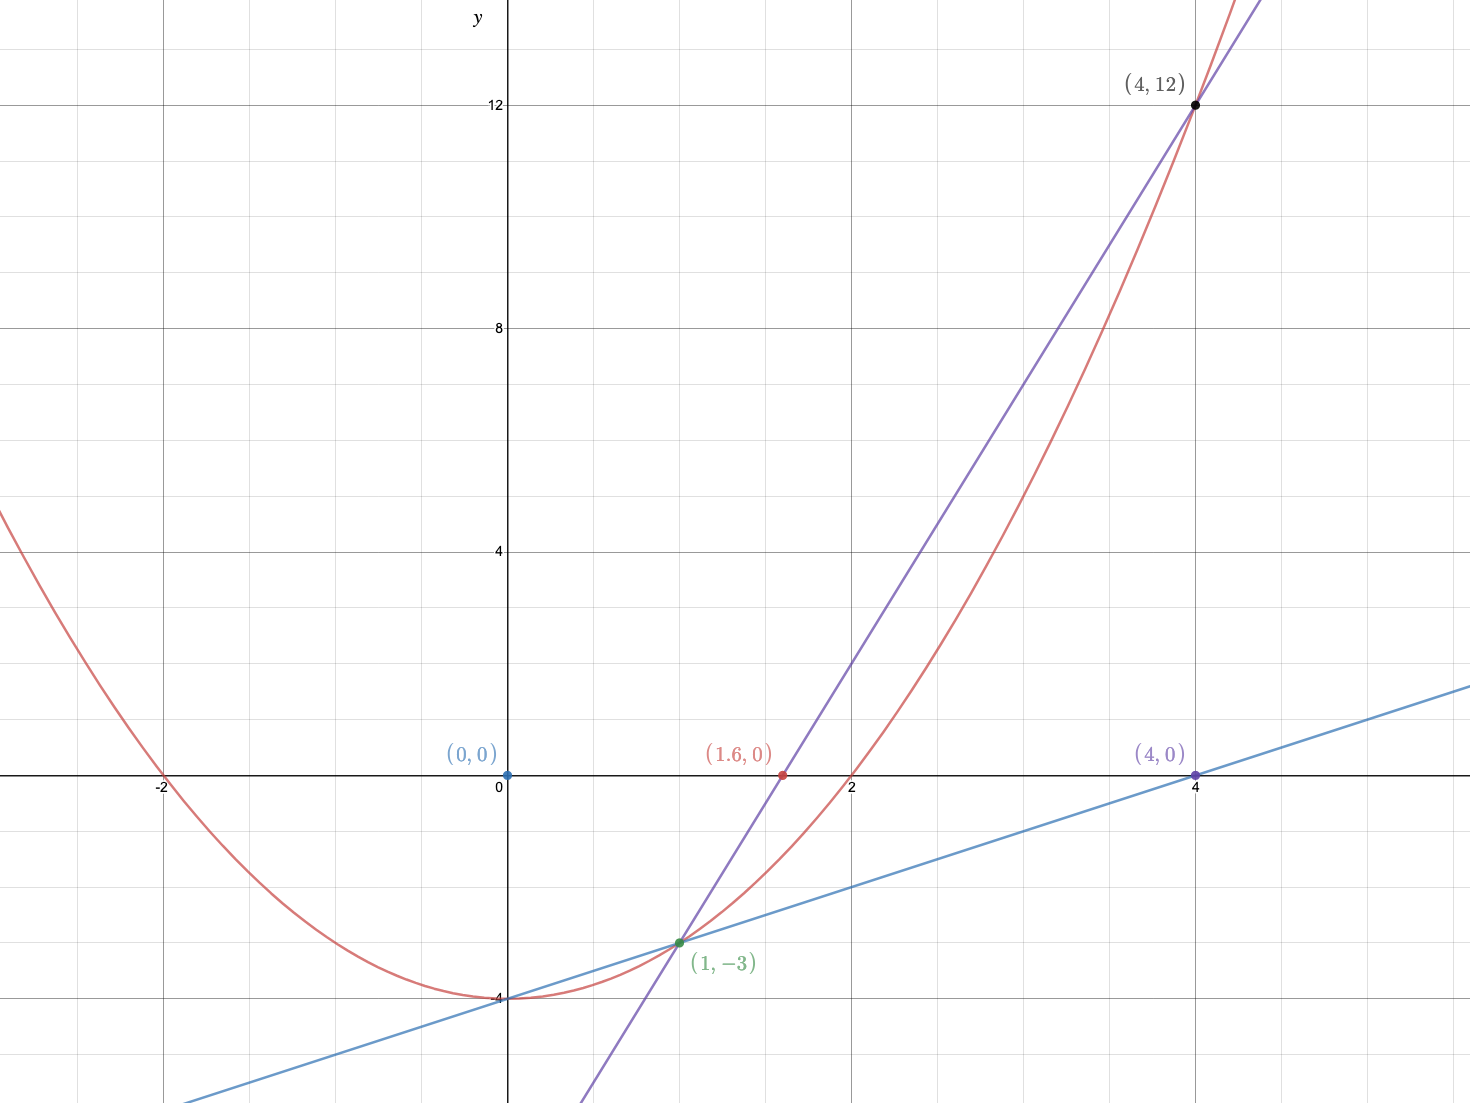
\includegraphics[width=\textwidth]{parab.png}
	\end{center}
\end{solution}

\begin{problem}
\begin{parts}
	\part{Show that the secant error $\epsilon_k$ for finding a simple root $x^*$ of $f(x)$ ($\epsilon_k = x_k - x^*$), to leading order, decays like \[\epsilon_{k+1} = \epsilon_k\epsilon_{k-1}\frac{f''(x^*)}{2f'(x^*)}.\]}\label{part:11a}
	\part{Consider the sequence $\{\abs{\epsilon_0}, \abs{\epsilon_1}, \abs{\epsilon_2},\ldots\}$ generated by Equation (2), and find a solution of the form \[\abs{\epsilon_{k+1}} = c\abs{\epsilon_k}^d\] for certain constants $c$ and $d$ that you are asked to compute (choose the relevant value of $d$ that must occur near convergence). Conclude about the order of convergence of the secant method.}\label{part:11b}
\end{parts}
\end{problem}

\begin{solution}
	\ref{part:11a}
	First, we will take $x^* = 0$. We then have the correspondence $\epsilon_k = x_k$ which allows us to write the secant method iteration scheme as
	\begin{equation*}
		\epsilon_{k+1} = \epsilon_k - f(\epsilon_k)\frac{\epsilon_k - \epsilon_{k-1}}{f(\epsilon_k) - f(\epsilon_{k-1})}.
	\end{equation*}
	Now we need to bring in the first a second derivatives of $f$ so we'll start by Taylor expanding.
	\begin{align*}
		f(\epsilon_k)                     & = f(0) + f'(0)\epsilon_k + f''(0)\frac{\epsilon_k^2}{2} + \order{\epsilon_k^3}                     \\
		                                  & \approx f'(0)\epsilon_k + f''(0)\frac{\epsilon_k^2}{2}                                             \\
		f(\epsilon_k) - f(\epsilon_{k-1}) & = \qty(\epsilon_k - \epsilon_{k-1})\qty[f'(0) + \qty(\epsilon_k + \epsilon_{k-1})\frac{f''(0)}{2}]
	\end{align*}
	Now let's plug these into the above iteration scheme and do algebra\ldots
	\begin{align*}
		\epsilon_{k+1} & = \epsilon_k - \frac{f'(0)\epsilon_k + f''(0)\frac{\epsilon_k^2}{2}}{f'(0) + \qty(\epsilon_k + \epsilon_{k-1})\frac{f''(0)}{2}}                                                   \\
		               & = \frac{1}{f'(0) + \qty(\epsilon_k + \epsilon_{k-1})\frac{f''(0)}{2}}\qty[\frac{\epsilon_k^2}{2}f''(0) + \frac{\epsilon_k\epsilon_{k-1}}{2}f''(0) - f''(0)\frac{\epsilon_k^2}{2}] \\
		               & = \frac{\frac{\epsilon_k\epsilon_{k-1}}{2}f''(0)}{f'(0) + \qty(\epsilon_k + \epsilon_{k-1})\frac{f''(0)}{2}}                                                                      \\
		               & = \frac{\epsilon_k\epsilon_{k-1}\frac{f''(0)}{2f'(0)}}{1 + \qty(\epsilon_k + \epsilon_{k-1})\frac{f''(0)}{2f'(0)}}                                                                \\
		               & \approx \epsilon_k\epsilon_{k-1}\frac{f''(0)}{2f'(0)} = \epsilon_k\epsilon_{k-1}\frac{f''(x^*)}{2f'(x^*)}
	\end{align*}

	\ref{part:11b}
	Now we want $\abs{\epsilon_{k+1}} = c\abs{\epsilon_k}^d$ and we know $\epsilon_{k+1} = \epsilon_k\epsilon_{k-1}C$ where $C = \frac{f''(x^*)}{2f'(x^*)}$.
	\begin{align*}
		\abs{\epsilon_{k+1}} = c\abs{\epsilon_k}^d & = \abs{\epsilon_k}\abs{\epsilon_{k-1}}\abs{C}                           \\
		\abs{\epsilon_k}^{d-1}                     & = \abs{\epsilon_{k-1}}\abs{\frac{C}{c}}                                 \\
		\abs{\epsilon_k}                           & = \abs{\epsilon_{k-1}}^{\frac{1}{d-1}}\abs{\frac{C}{c}}^{\frac{1}{d-1}}
	\end{align*}
	Thus $d = \frac{1}{d - 1}$ which has solutions $d = \frac{1\pm\sqrt{5}}{2}$, but we know $d$ must be greater than 0 in order for convergence to happen, so $d = \frac{1 + \sqrt{5}}{2}$ also known as the golden ratio $\varphi$! Cool. Similarly for the constant $c$ we have
	\begin{align*}
		c               & = \abs{\frac{C}{c}}^{\varphi}                             \\
		c^{\varphi + 1} & = \abs{\frac{f''(x^*)}{2f'(x^*)}}                         \\
		c               & = \abs{\frac{f''(x^*)}{2f'(x^*)}}^{\frac{1}{\varphi + 1}}
	\end{align*}
	Lastly we have
	\begin{equation*}
		\abs{\epsilon_k} = \abs{\frac{f''(x^*)}{2f'(x^*)}}^{\frac{1}{\varphi + 1}}\abs{\epsilon}^\varphi
	\end{equation*}
	so we conclude that this method converges faster than linear, but not quite quadratically.
\end{solution}

\begin{problem}
Consider the root finding method
\[x_{k+1} = x_k - \frac{2f(x_k)f'(x_k)}{2f'(x_k)^2 - f(x_k)f''(x_k)}.\]
Rewrite this method as a fixed point method $x_{k+1} = \phi(x_k)$. Find the order of convergence for this method (for a simple root). Derive an expression for the asymptotic error constant. (You can assume that $f(x)$ has continuous derivatives of any required order.)
\end{problem}

\begin{solution}
	First define the following function:
	\begin{equation*}
		\phi(x) = x - \frac{2f(x)f'(x)}{2f'(x)^2 - f(x)f''(x)}.
	\end{equation*}
	Clearly we have $\phi(x_k) = x_{k+1}$ by using our root finding method. To find the order of convergence I'm pretty stuck. I've tried writing $f(x)$ as a Taylor series and expanding out the entire formula to the lowest degree term, but it becomes extremely messy, and I'm not sure that's the right approach to begin with. I do feel like I can make an educated guess about he order of convergence, but it's really not that strong: because the method is much more complicated than Newton's method (and takes into account more information than just the first derivative at a point), it's order of convergence must be greater than that of Newton's method (otherwise what's the point of throwing in all that extra information). So I might guess the order is qubic quartic, or maybe any $p\in(2, 3)$, where I doubt it could be higher than 4 since there are no third derivatives.
\end{solution}


\end{document}
